\documentclass{article}

\usepackage[T1]{fontenc}
\usepackage[utf8]{inputenc}
\usepackage[french]{babel}
\usepackage[affil-it]{authblk}
\usepackage{fullpage}
\usepackage{graphicx}
\usepackage{biblatex}

\usepackage{multirow}
\usepackage[table,xcdraw]{xcolor}

\usepackage{stackengine}
\usepackage{listings}
\usepackage{glossaries}
\makeglossaries

\newenvironment*{remerciements}{%
  \renewcommand*{\abstractname}{Remerciements}
  \begin{abstract}
}{
  \end{abstract}
}

\bibliography{introduction/sources}
\bibliography{centralisation/sources}
\bibliography{decentralisation/sources}


\begin{document}

\title{Echange de jetons inter-blockchains}
\author{VOLPE Dorian, ROTONDO Eloïse, TESTUD Romain,\\DE CAMPOU Louis, JOLY Amaury  \\ \textbf{Encadrants :} TRAVERS Corentin, LABOUREL Arnaud \\ 
\includegraphics[scale=0.1]{./img/amu.png}}
\affil{Aix-Marseille Université, M2 Fiabilité et sécurité informatique}
\date{\today}

\begin{titlepage}
  \maketitle
\end{titlepage}

\begin{remerciements}
  Merci à M. TRAVERS Corentin et M. LABOUREL Arnaud pour la proposition de ce sujet et son encadrement.
\end{remerciements}
\begin{abstract}
  Ces dernières années, un grand nombre de blockchains ont vu le jour, accompagnées d’un lot de problématiques.
  Parmi les questions les plus importantes figure celle des échanges entre ces blockchains.
  En effet le marché des cryptomonnaies augmente fortement et malheureusement toutes les blockchains ne sont pas forcément compatibles entre elles, ce qui crée une forte pression sur le marché actuel.
  Dans cet ouvrage, vous trouverez un résumé exhaustif des recherches menées sur les échanges cross-chain.
  Que ce soit en termes de protocoles ou bien d'implémentation plus techniques, nous avons essayé de regrouper le plus grand nombre d'exemples.
  Nous commencerons par les protocoles d’échanges centralisés qui sont les plus répandus grâce à leur facilité d'utilisation et leur rapidité.
  Mais ces protocoles sont souvent la source d'attaques ou bien même de failles, car le marché des échanges inter-blockchain est souvent rejoint par des entités n'ayant pas de connaissance en fiabilité.
  Ensuite nous continuerons par les protocoles d'échanges décentralisés qui représentent une bonne alternative aux échanges centralisés, car ils offrent une meilleure sécurité au détriment d'une complexité d'utilisation accrue.
  Vous allez donc pouvoir comprendre quels sont les avantages et les inconvénients de ces deux méthodes d'échanges de jetons inter-blockchain.
\end{abstract}

\newpage

\tableofcontents

\newpage

\section{Introduction}
\begin{frame}{Centralisé}
    \begin{block}{Le centralisé offre\dots}
        \begin{itemize}
            \item Diversité d'acteurs.
            \item Accessibilité.
            \item Multiples fonctionnalités.
        \end{itemize}
    \end{block}
    \pause
    \begin{block}{Mais\dots}
        \begin{itemize}
            \item Opacité des protocoles.
            \item Failles de sécurité.
            \item Collecte des données.
        \end{itemize}
    \end{block}
\end{frame}


\begin{frame}{Décentralisé}
    \begin{block}{Le décentralisé offre\dots\dots}
        \begin{itemize}
            \item Pas de tiers de confiance.
            \item Transparence.
            \item Fiabilité accrue.
        \end{itemize}
    \end{block}
    \pause
    \begin{block}{Mais\dots}
        \begin{itemize}
            \item Difficiles d'accès.
            \item Intérêt économique faible.
        \end{itemize}
    \end{block}
\end{frame}

\begin{frame}{Conclusion générale}
    \begin{itemize}
        \item Flou entre centralisé/décentralisé.
        \item Définition variable.
    \end{itemize}
\end{frame}

\begin{frame}
    \begin{figure}
        \begin{figure}
            \centering
            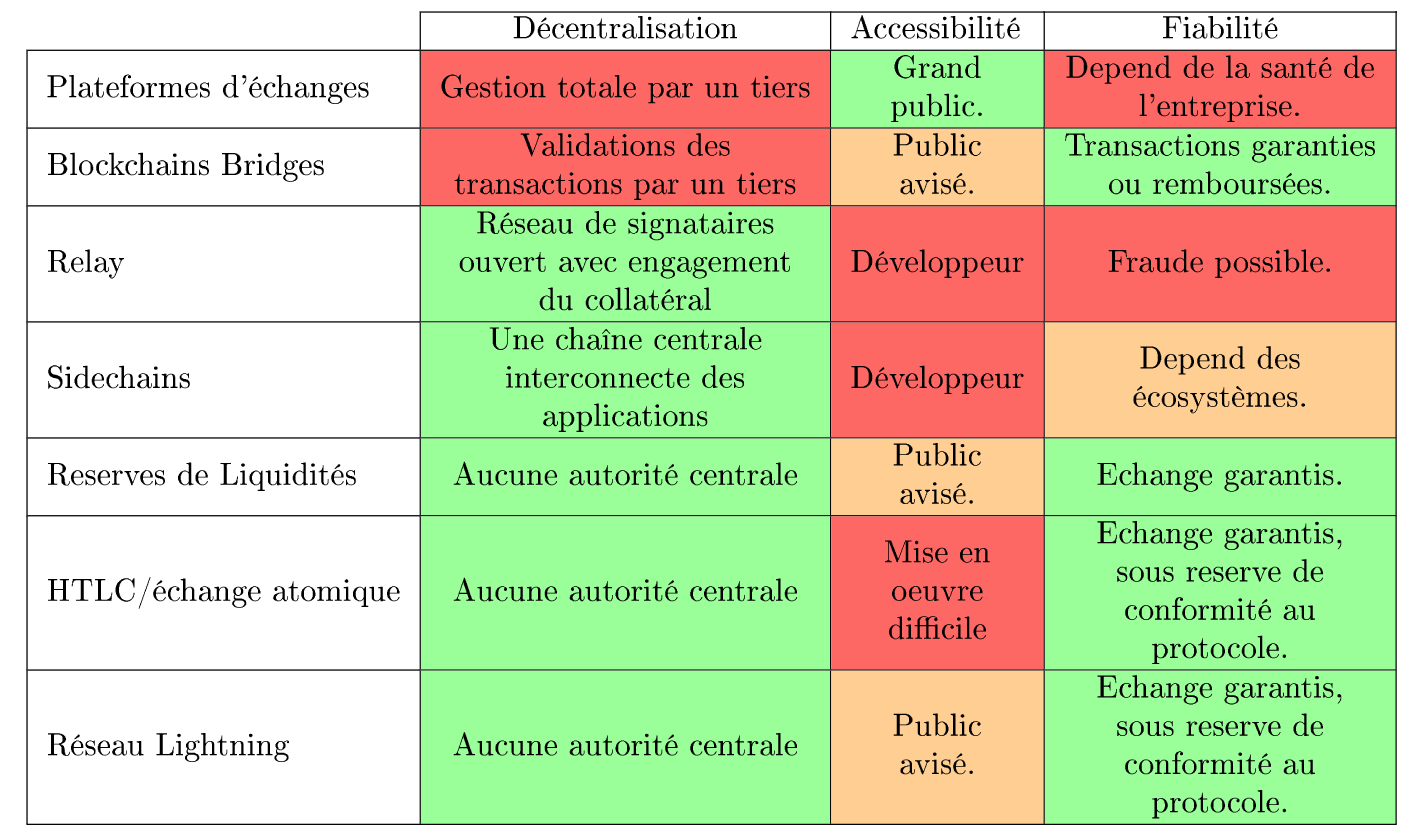
\includegraphics[scale = 0.2]{conclusion/tableau.png}
            \label{fig:recap}
            \caption{Tableau récapitulatif}
        \end{figure}
    \end{figure}
    
\end{frame}

\newpage

\newglossaryentry{dApp}{
    name = dApp,
    description= {abréviation de "application décentralisée". C’est une application qui fonctionne sur une blockchain ou
            tout autre registre décentralisé public et qui est conçu pour être autonome et transparent}
}

\newglossaryentry{cross-chain}{
    name = cross-chain,
    description= {Les échanges cross-chain sont des échanges entre plusieurs blockchains.
            Un participant utilise ses actifs dans une \textit{blockchain} pour échanger les actifs d’autres personnes dans différentes \textit{blockchains}}
}

\newglossaryentry{actif}{
    name = actif,
    description= {Dans le contexte de la \textit{blockchain}, un actif ou jeton peut être matériel (une maison, une voiture, de l’argent, un terrain) ou immatériel (propriété intellectuelle, brevets, droits d’auteur, marque).
            Tout ce qui a de la valeur est traçable et échangeable sur un réseau de blockchain}
}

\newglossaryentry{smart contract}{
    name = smart contract,
    description= {Un smart contract est une application décentralisée qui exécute automatiquement des instructions prédéfinies lorsqu’il est déployé sur une \textit{blockchain}.}
}

\newglossaryentry{blockchain}{
    name = blockchain,
    description= {Une \textit{blockchain} est une base de données distribuée avec une liste (c'est-à-dire une chaîne) d'enregistrements (c'est-à-dire des blocs) liés et sécurisés par des empreintes numériques (c'est-à-dire des hachages crypto)}
}

\printglossaries

\newpage
\section{Systèmes Centralisés}
\begin{frame}{Centralisé}
    \begin{block}{Le centralisé offre\dots}
        \begin{itemize}
            \item Diversité d'acteurs.
            \item Accessibilité.
            \item Multiples fonctionnalités.
        \end{itemize}
    \end{block}
    \pause
    \begin{block}{Mais\dots}
        \begin{itemize}
            \item Opacité des protocoles.
            \item Failles de sécurité.
            \item Collecte des données.
        \end{itemize}
    \end{block}
\end{frame}


\begin{frame}{Décentralisé}
    \begin{block}{Le décentralisé offre\dots\dots}
        \begin{itemize}
            \item Pas de tiers de confiance.
            \item Transparence.
            \item Fiabilité accrue.
        \end{itemize}
    \end{block}
    \pause
    \begin{block}{Mais\dots}
        \begin{itemize}
            \item Difficiles d'accès.
            \item Intérêt économique faible.
        \end{itemize}
    \end{block}
\end{frame}

\begin{frame}{Conclusion générale}
    \begin{itemize}
        \item Flou entre centralisé/décentralisé.
        \item Définition variable.
    \end{itemize}
\end{frame}

\begin{frame}
    \begin{figure}
        \begin{figure}
            \centering
            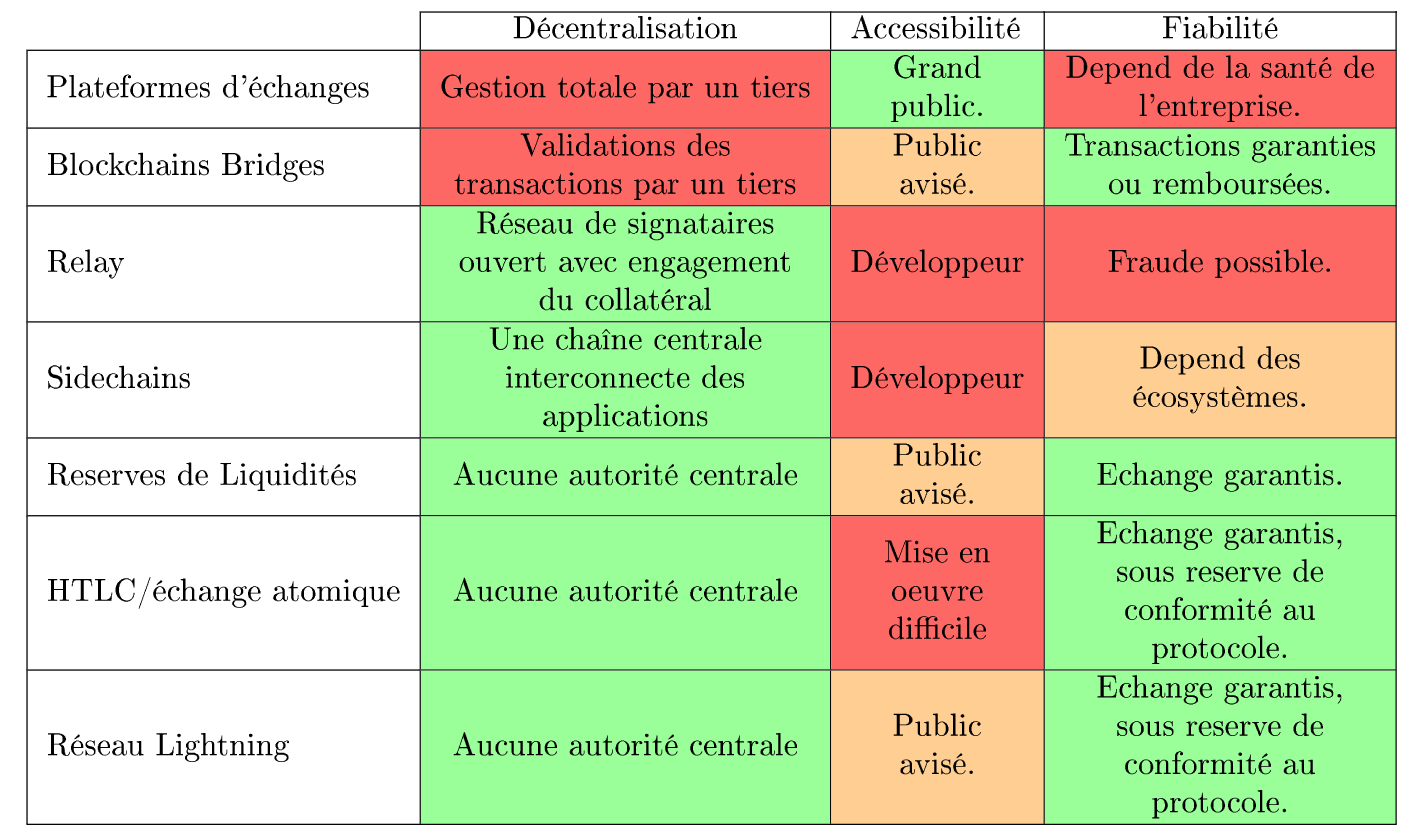
\includegraphics[scale = 0.2]{conclusion/tableau.png}
            \label{fig:recap}
            \caption{Tableau récapitulatif}
        \end{figure}
    \end{figure}
    
\end{frame}

\newpage
\section{Systèmes Décentralisés}
\begin{frame}{Centralisé}
    \begin{block}{Le centralisé offre\dots}
        \begin{itemize}
            \item Diversité d'acteurs.
            \item Accessibilité.
            \item Multiples fonctionnalités.
        \end{itemize}
    \end{block}
    \pause
    \begin{block}{Mais\dots}
        \begin{itemize}
            \item Opacité des protocoles.
            \item Failles de sécurité.
            \item Collecte des données.
        \end{itemize}
    \end{block}
\end{frame}


\begin{frame}{Décentralisé}
    \begin{block}{Le décentralisé offre\dots\dots}
        \begin{itemize}
            \item Pas de tiers de confiance.
            \item Transparence.
            \item Fiabilité accrue.
        \end{itemize}
    \end{block}
    \pause
    \begin{block}{Mais\dots}
        \begin{itemize}
            \item Difficiles d'accès.
            \item Intérêt économique faible.
        \end{itemize}
    \end{block}
\end{frame}

\begin{frame}{Conclusion générale}
    \begin{itemize}
        \item Flou entre centralisé/décentralisé.
        \item Définition variable.
    \end{itemize}
\end{frame}

\begin{frame}
    \begin{figure}
        \begin{figure}
            \centering
            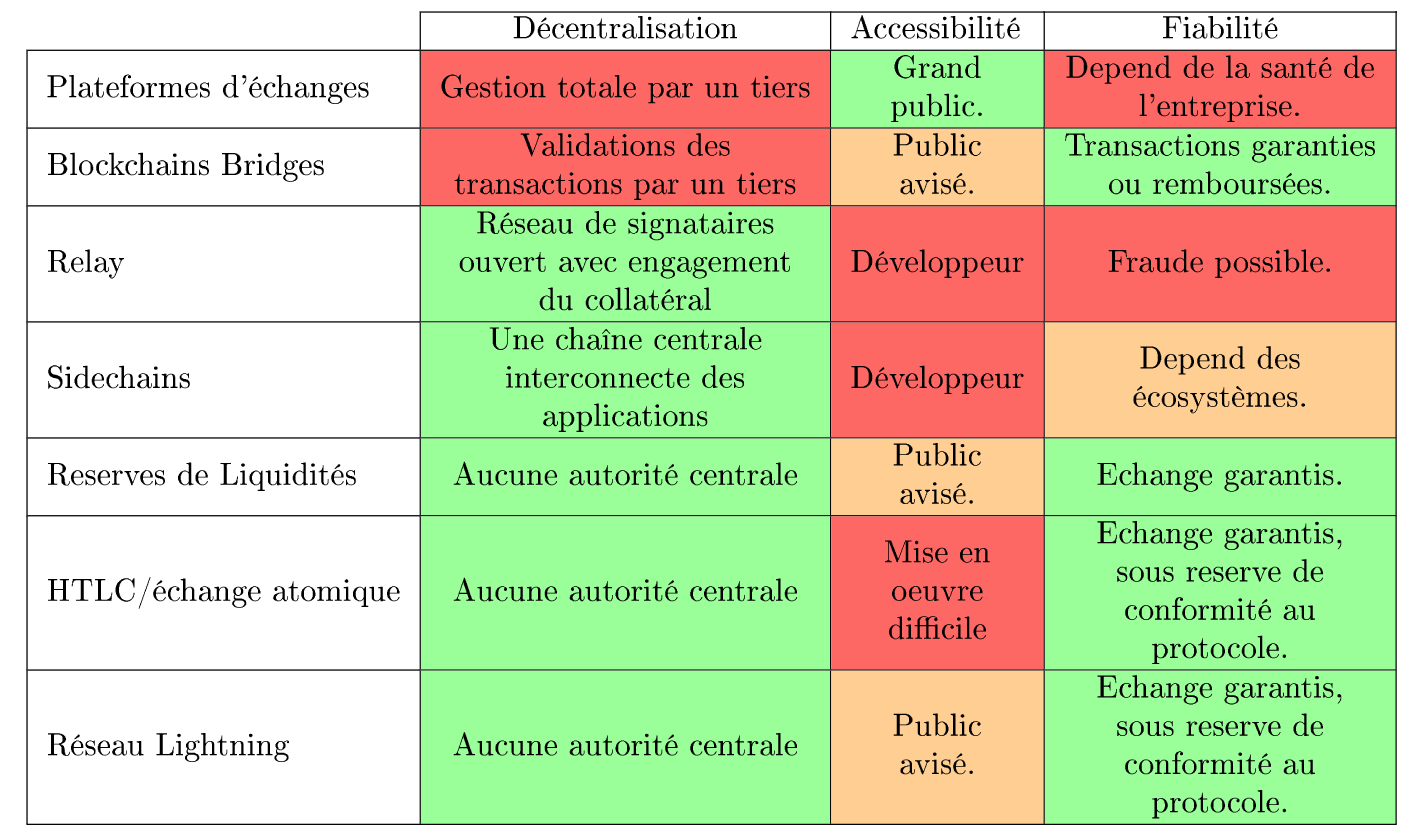
\includegraphics[scale = 0.2]{conclusion/tableau.png}
            \label{fig:recap}
            \caption{Tableau récapitulatif}
        \end{figure}
    \end{figure}
    
\end{frame}

\newpage

\section{Conclusion}
\begin{frame}{Centralisé}
    \begin{block}{Le centralisé offre\dots}
        \begin{itemize}
            \item Diversité d'acteurs.
            \item Accessibilité.
            \item Multiples fonctionnalités.
        \end{itemize}
    \end{block}
    \pause
    \begin{block}{Mais\dots}
        \begin{itemize}
            \item Opacité des protocoles.
            \item Failles de sécurité.
            \item Collecte des données.
        \end{itemize}
    \end{block}
\end{frame}


\begin{frame}{Décentralisé}
    \begin{block}{Le décentralisé offre\dots\dots}
        \begin{itemize}
            \item Pas de tiers de confiance.
            \item Transparence.
            \item Fiabilité accrue.
        \end{itemize}
    \end{block}
    \pause
    \begin{block}{Mais\dots}
        \begin{itemize}
            \item Difficiles d'accès.
            \item Intérêt économique faible.
        \end{itemize}
    \end{block}
\end{frame}

\begin{frame}{Conclusion générale}
    \begin{itemize}
        \item Flou entre centralisé/décentralisé.
        \item Définition variable.
    \end{itemize}
\end{frame}

\begin{frame}
    \begin{figure}
        \begin{figure}
            \centering
            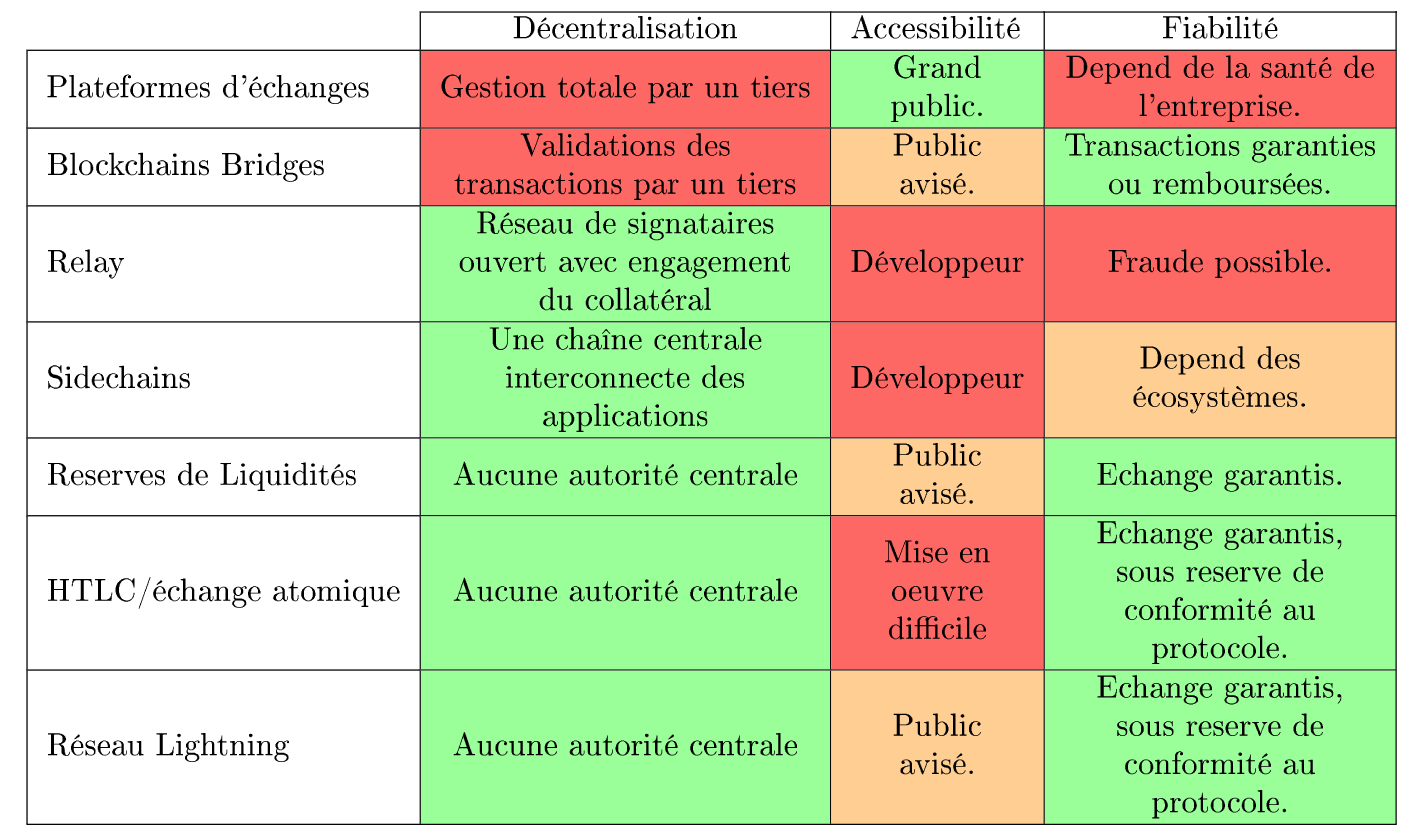
\includegraphics[scale = 0.2]{conclusion/tableau.png}
            \label{fig:recap}
            \caption{Tableau récapitulatif}
        \end{figure}
    \end{figure}
    
\end{frame}

\newpage

\printbibliography

\end{document}
